\subsection{Online nesting experiment} \label{subsec:nest_online}
%----------------------------------------------------------

The following two limitations are imposed in carrying out the online nesting experiment:
\begin{itemize}
\item The integration time for the child domain is identical to that for the parent domain.
\item The time step for the parent domain is a multiple of that for the child domain.
\end{itemize}
On the other hand, the configurations of vertical layers, map projections, and the physical scheme do not have to be identical in the parent and the child domains. In the online nesting experiment, computations of all domains are conducted simultaneously. In the current version, \scalerm supports only one-way nesting. The maximum number of domains allowed is 10.

In the online nesting experiment in \scalerm, the time integrations of multiple domains are not serial but parallel. As shown in Fig. \ref{fig_mpisplit}, MPI processes are split into several groups; each group manages a domain and computes it, behaving like an independent model. The configuration file \verb|launch.conf| is needed at execution to boot the multiple domains.

\begin{figure}[tbh]
\begin{center}
  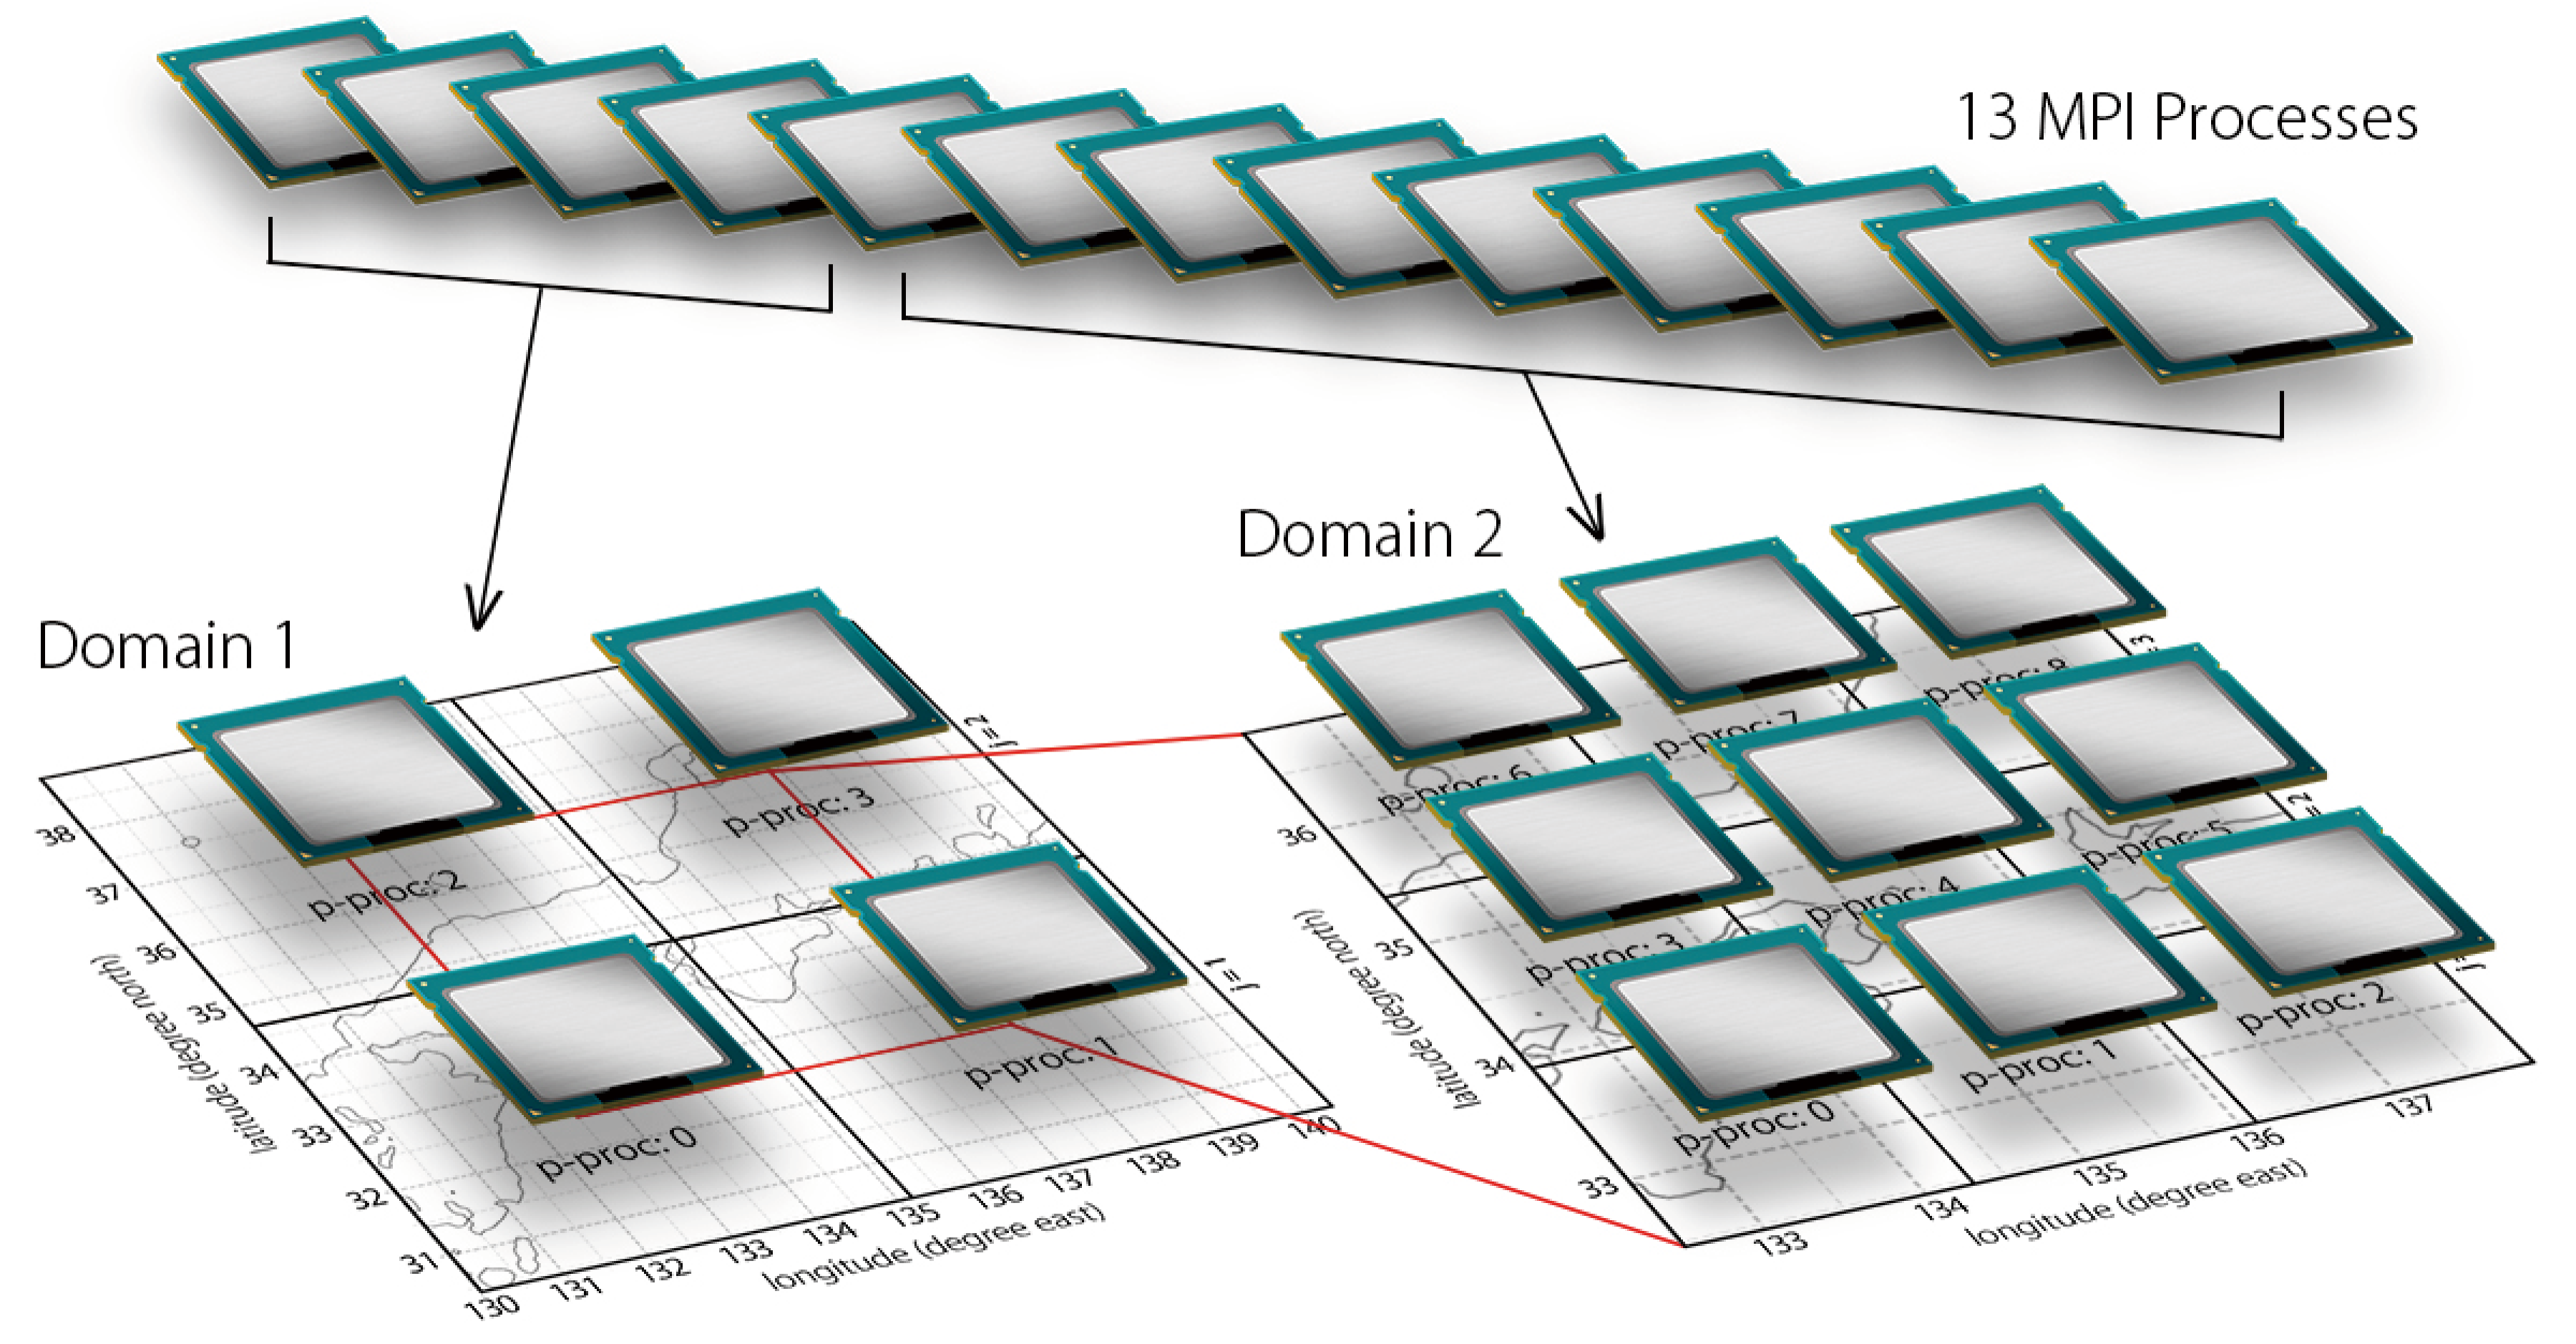
\includegraphics[width=0.8\hsize]{./figure/mpisplit_nesting.png}\\
  \caption{ MPI process distribution in the online nesting experiment. In this example,   13 processes were launched at the beginning. These processes were distributed appropriately;     4-MPI parallel for $2 \times 2$ in Domain 1 and 9-MPI parallel for $3 \times 3$ in Domain 2 were executed.     MPI communication flowed from Domain 1 to Domain 2.
  }
  \label{fig_mpisplit}
\end{center}
\end{figure}

The following explanation is provided for the most simple case of online nesting, two-domain nesting.
The experimental set described here can be generated by renaming the sample files \\
\verb|${Tutorial_dir}/real/sample/USER.online-nesting.sh|
as USER.sh and conducting ``the making tool for the complete settings of the experiment'' ( refer to Section \ref{sec:basic_makeconf} ).
The below explanation assumes that the generations of the topography/land-use data and initial/boundary data for each domainhave been completed. The procedures for topography generation are described in Section \ref{subsec:nest_topo}.


\subsubsection{Editing the configuration file}
In the configuration files \verb|run.***.conf| for the parent and child domains, some nesting settings are added to \namelist{PARAM_NEST}:

\noindent {\rm --- Configuration in \verb|run.d01.conf| ---}\\
\editboxtwo{
\verb|&PARAM_NEST|                          & \\
\verb| ONLINE_DOMAIN_NUM        = 1,      | & The domain ID, which is enumerated from the outermost one as 1.\\
\verb| ONLINE_IAM_PARENT        = .true., | & \\
\verb| ONLINE_IAM_DAUGHTER      = .false.,| & \\
\verb| ONLINE_BOUNDARY_USE_QHYD = .true., | & \\
\verb| ONLINE_AGGRESSIVE_COMM   = .true., | & \\
\verb|/| \\
}
~\\
\noindent {\rm --- Configuration in \verb|run.d02.conf| ---}\\
\editboxtwo{
\verb|&PARAM_NEST| & \\
\verb| ONLINE_DOMAIN_NUM        = 2,      | & The domain ID, which is enumerated from the outermost one as 1.\\
\verb| ONLINE_IAM_PARENT        = .false.,| & \\
\verb| ONLINE_IAM_DAUGHTER      = .true., | & \\
\verb| ONLINE_BOUNDARY_USE_QHYD = .true., | & \\
\verb| ONLINE_AGGRESSIVE_COMM   = .true., | & \\
\verb|/| \\
}

\nmitem{ONLINE_DOMAIN_NUM} is the ID number of the domain, which is enumerated from the outermost domain to the innermost.
In above example, the ID numbers of the parent and child domains are 1 and 2, respectively.\\
\nmitem{ONLINE_IAM_PARENT} and \nmitem{ONLINE_IAM_DAUGHTER} specify whether each domain has its parent domain and child domain or not.
If \nmitem{ONLINE_IAM_PARENT} $=$ \verb|.true.| in the Nth domain, the calculation data in the Nth domain is transferred to the child domain with the domain number of N+1.
If \nmitem{ONLINE_IAM_DAUGHTER} $=$ \verb|.true.|, then boundary data in the Nth domain is received from the parent with the domain number of N-1.
The outermost domain plays a role only in the parent domain, whereas the innermost domain is involved only in the child domain.
Since the intermediate domains are involved in both the parent and child domains, both \nmitem{ONLINE_IAM_PARENT} and \nmitem{ONLINE_IAM_DAUGHTER} are \verb|.true.|.
Table \ref{tab:triple_nested} gives the configuration for an N-domain nesting experiment.

\begin{table}[htb]
\begin{center}
\caption{A configuration for N-domain nesting}
\begin{tabularx}{150mm}{|l|l|l|X|} \hline
 \rowcolor[gray]{0.9} domain & \verb|ONLINE_DOMAIN_NUM| & \verb|ONLINE_IAM_PARENT| & \verb|ONLINE_IAM_CHILD|\\ \hline
 the outermost domain & 1          & .true.  & .false. \\ \hline
 intermediate domains & 2 -- (N-1) & .true.  & .true. \\ \hline
 the innermost domain & N          & .false. & .true. \\ \hline
\end{tabularx}
\label{tab:triple_nested}
\end{center}
\end{table}


\nmitem{ONLINE_BOUNDARY_USE_QHYD} specifies whether water condensation is used for the boundary condition. When the boundary condition is generated from external input data, water condensations are not usually employed. However, in the nesting experiment, water condensation calculated in the parent domain can be used for the boundary condition of the child domain because there is often no difference in physical schemes between the two domains.
%, and the resolution of both are similar.
The delay in the generation of clouds and rain, as influence on the target domain, is expected to be suppressed by this remedy.

\subsubsection{Configuration of launch file}
\label{subsubsec:launch}
The online nesting experiment requires the configuration of the launch file \verb|launch.conf|
other than \verb|run.***.conf|.
\editboxtwo{
\verb|&PARAM_LAUNCHER|      & \\
\verb| NUM_DOMAIN  = 2,|    & number of domains\\
\verb| PRC_DOMAINS = 4, 16,| & MPI processes used for each domain (as many domains as necessary)\\
\verb| CONF_FILES  = run.d01.conf, run.d02.conf,| & The configuration files for each domain (as many domains as necessary)\\
\verb|/|& \\
}
\nmitem{CONF_FILES} must correspond to \nmitem{PRC_DOMAINS} in order.
The above case means that
the run is executed by
the 4-MPI parallel for the parent domain 
and the 16-MPI parallel for the child domain;
each number of processes in the launch file 
must correspond to the total number of MPI processes ( \verb|PRC_NUM_X|$\times$\verb|PRC_NUM_Y| )
specified in each configuration file \verb|run.***.conf|.

At execution, the total number of MPI processes is given, which different from that in the case of single-domain execution. For example, 20 processes are specified in the above case.
\begin{verbatim}
 $ mpirun  -n  [number of processes]  ./scale-rm  launch.conf
\end{verbatim}

When multiple domain calculations are executed at the same time,
the different file names must be used for input/output files
among domains to avoide any confusion.
For example, the configuration files prepared by the 
``the making tool for the complete settings of the experiment''
use \verb|history_d01.pe***.nc, history_d02.pe***.nc| for the file name of history output.

The calculation may sometimes abort, outputting the message below. This is the error message, meaning that the domain of computation of the child  is larger than that of the parent domain. If the error message indicates ``SW search,'' the western or southern area of the child domain is beyond the parent domain. If the error message indicates ``NE search,'' the eastern or northern area of the child domain is beyond the parent domain. If such a message appears, retry creating the topography, the land-use data, and the initial/boundary data, and confirm again whether the configurations are correct:
\msgbox{
\verb|xxx region of daughter domain is larger than that of parent: SW search| \\
}
\msgbox{
\verb|xxx region of daughter domain is larger than that of parent: NE search| \\
}


\subsubsection{Guideline for distribution of MPI processes}
%-------------------------------------------------------------------------

As shown in Fig. \ref{fig_mpisplit}, no MPI process is shared between the multiple domains in the online nesting experiment. In other words, each MPI process takes charge of a part of a specific domain. Therefore, the user should determine how many MPI processes to allocate to each domain. When this allocation is not appropriate, a long waiting time is incurred. To avoid this situation, it is reasonable to allocate processes such the magnitude of time integrations for each process is as similar in value as is possible among processes\footnote{More accurately, floating-point operations should be estimated.}. Here, the magnitude of time integration, i.e., computational effort, is defined as the product of the number of grids and time steps.

Let us consider N-domain nesting. The number of grids in the x, y, and z directions in n-th domain are denoted by
\verb|IMAX_n|, \verb|JMAX_n|, and \verb|KMAX_n|, respectively.
\verb|DT_n| is the time interval \nmitem{TIME_DT} in the n-th domain.
Using the time-step of the outermost domain (n=1) \verb|DT_1| as a benckmark, 
the necessary number of time steps in the n-th domain is estimated as:
\begin{eqnarray}
 \verb|TSTEP_n| = \verb|DT_1| / \verb|DT_n|  \nonumber
\end{eqnarray}
The calculation for the n-th domain is derived by multiplying the number of grids as
\begin{eqnarray}
 \verb|OPR_n| = \verb|IMAX_n| \times \verb|JMAX_n| \times \verb|KMAX_n| \times \verb|TSTEP_n| \nonumber
\end{eqnarray}
The standard number of processes allocated to the n-th domain is estimated as
\begin{eqnarray}
 \verb|MPI_total| \times \frac{ \texttt{OPR\_n} }{ \sum_{m=1}^N \texttt{OPR\_m} },
\end{eqnarray}
where \verb|MPI_total| is the total number of MPI processes.

The number of processes distributed along the x and y directions \nmitem{PRC_NUM_X, PRC_NUM_Y} can be arbitrarily decided.
It is recommended to configure them so that the difference between \verb|IMAX| and \verb|JMAX| is as small as possible. This is because such a configuration can reduce the area of the halo. As a result, high computational performance can be obtained\footnote{Note that in case of hybrid parallelization used together with thread parallelism,  e.g., in the K computer, it is necessary to take a larger number of grids along the y-axis than the x-axis to minimize computational imbalance between threads.}. 


In the above explanation, only the number of grids and time steps are considered. However, in actual calculations such as nesting simulation in real atmospheric experiment, the time interval for each physical process, and intra-domain and inter-domain communications affect the elapsed time. In the online nesting configuration, the calculation in the innermost domain is largest in general.  In case of large-scale computations, long integration and many ensemble simulations, it is recommended to tune for the distribution of processes following the above rough estimation.

